\begin{figure}
    % Number of observations NYALE13S
	\subfloat[\textcolor{black}{Number of observations - NYALE13S - Solution 0}.\label{fig:num-Ns-0}]
      {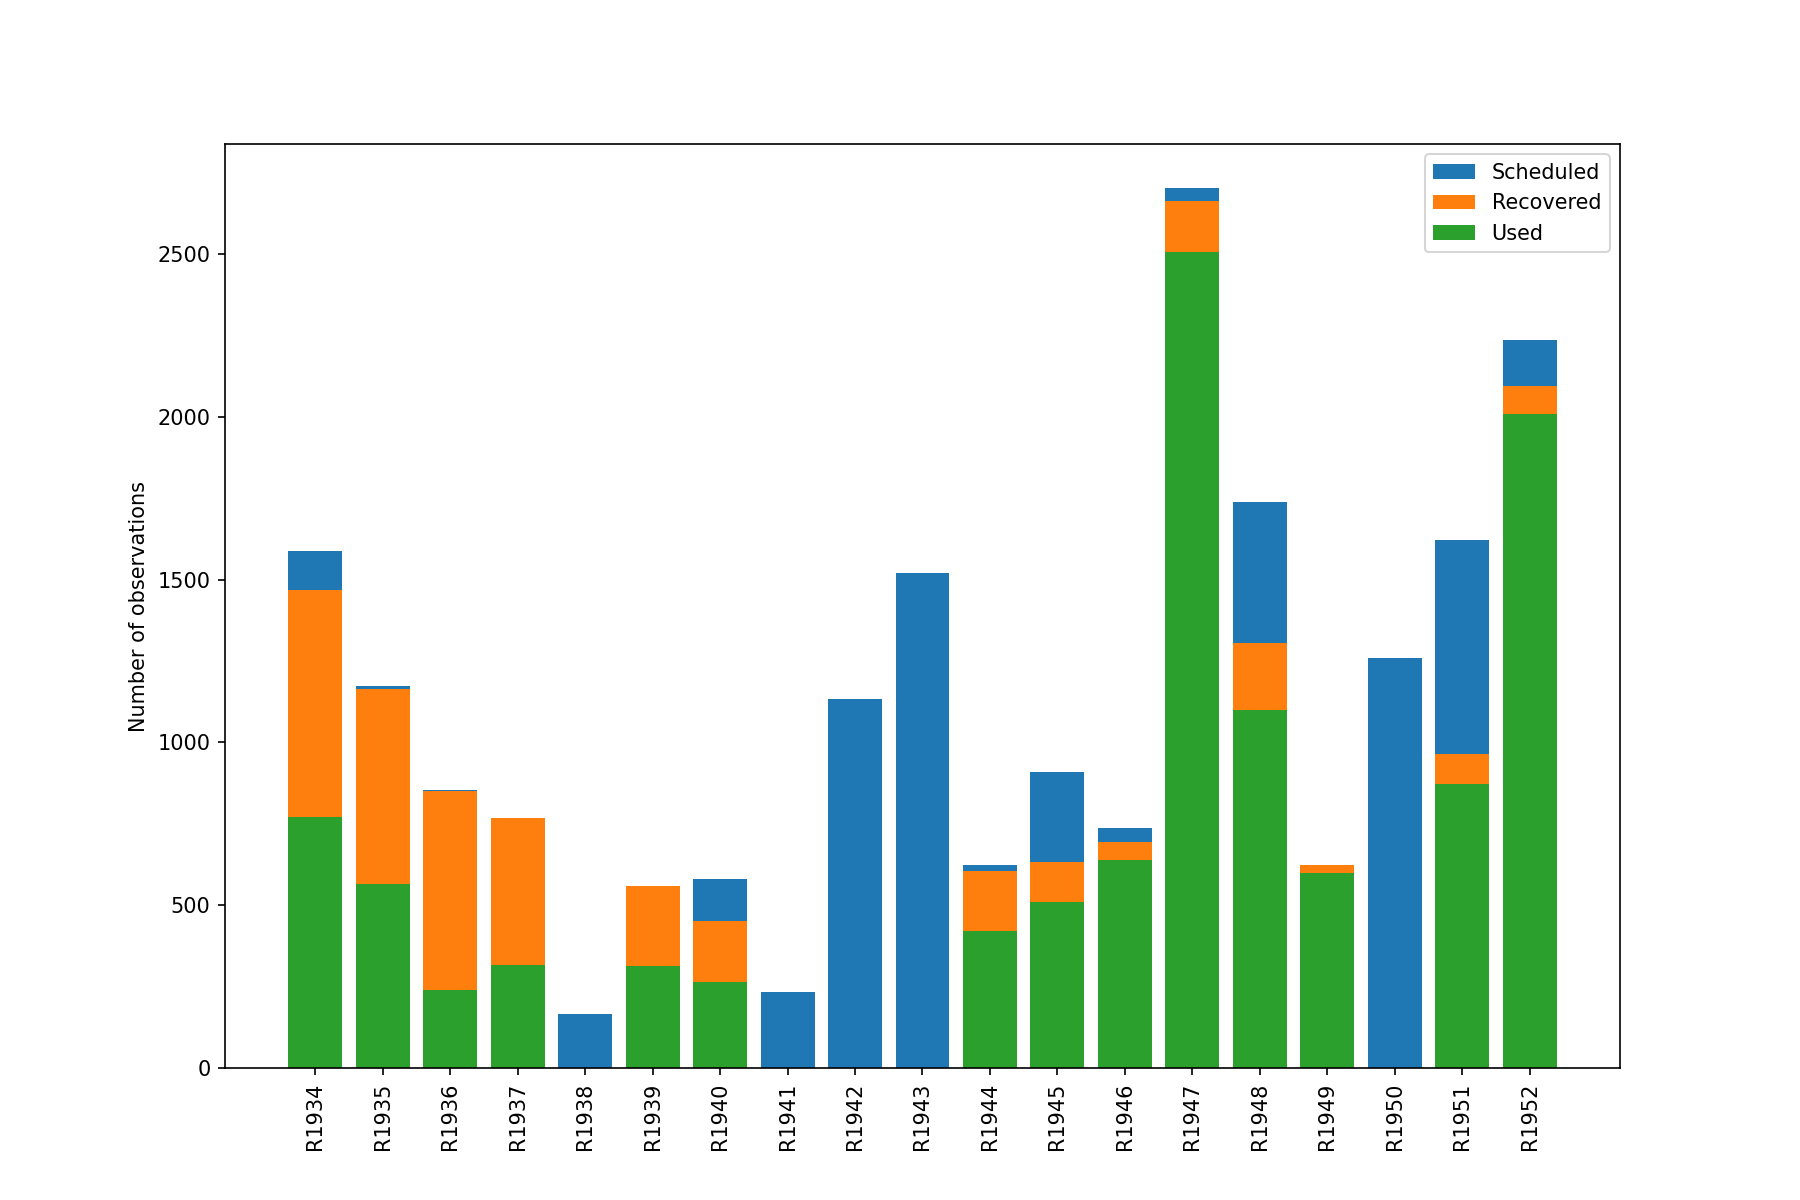
\includegraphics[width=0.5\linewidth]{figure/Num_obs_NYALE13S_nyale13s0}}
	\subfloat[\textcolor{black}{Number of observations - NYALE13S - Solution 9}.\label{fig:num_Ns-9}]
      {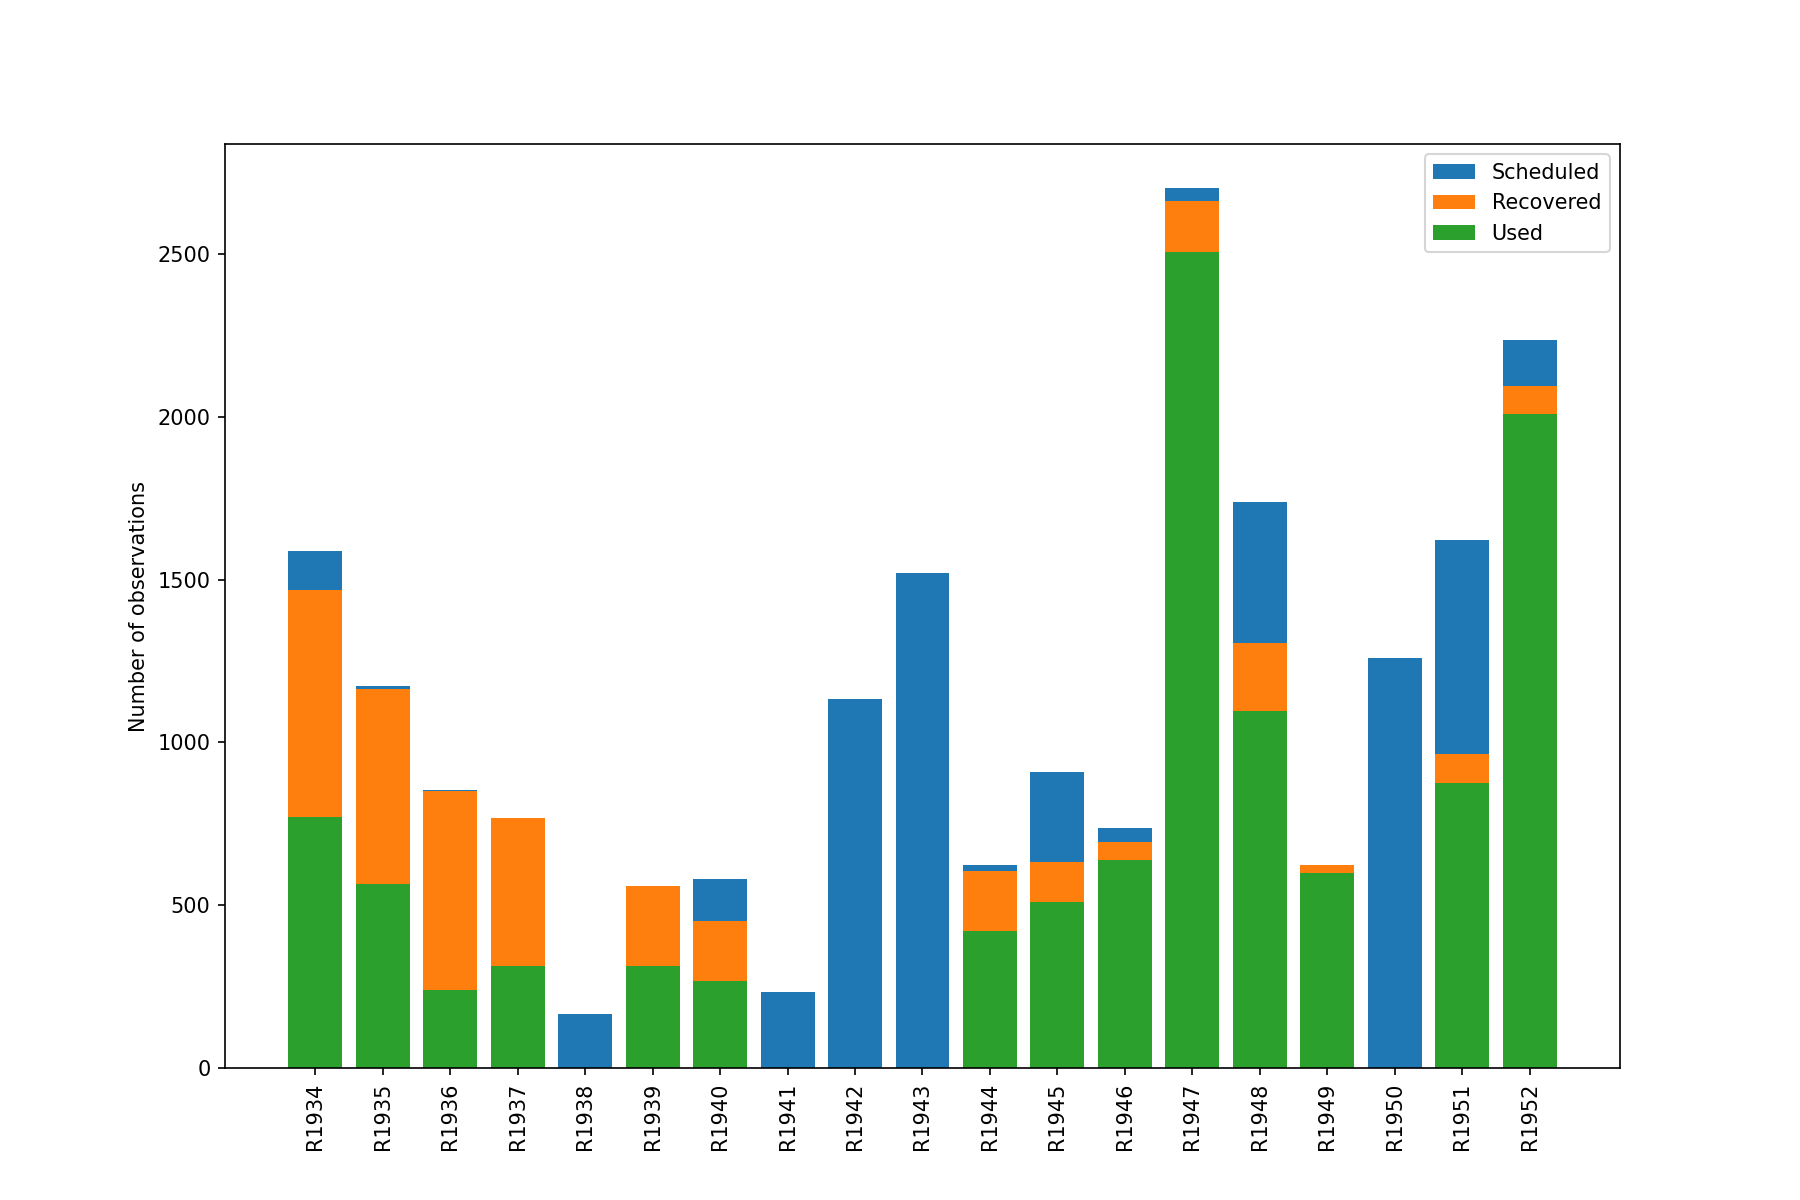
\includegraphics[width=0.5\linewidth]{figure/Num_obs_NYALE13S_nyale13s9}} \\
    % Number of observations NYALES20
	\subfloat[\textcolor{black}{Number of observations - NYALES20 - Solution 0}.\label{fig:num-Ny-0}]
      {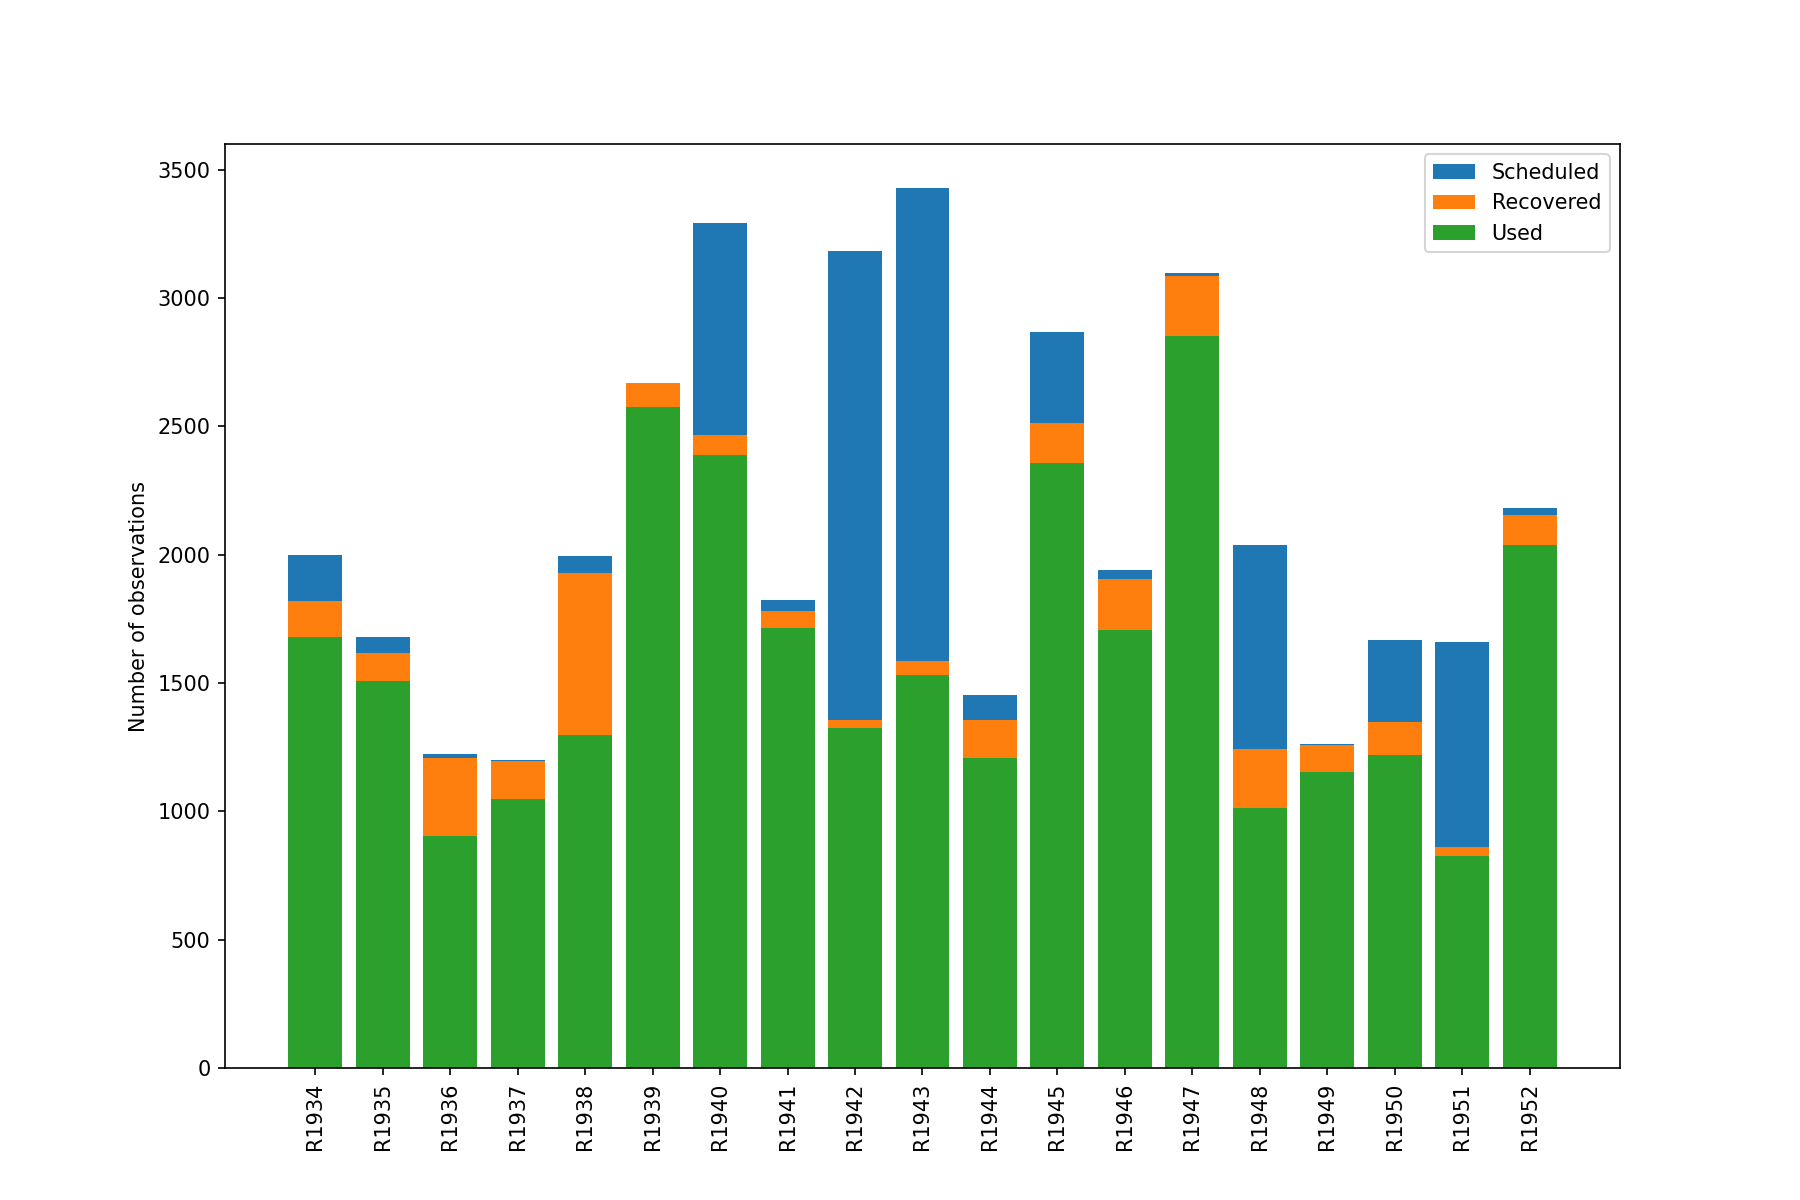
\includegraphics[width=0.5\linewidth]{figure/Num_obs_NYALES20_nyale13s0}}
	\subfloat[\textcolor{black}{Number of observations - NYALES20 - Solution 9}.\label{fig:num_Ny-9}]
      {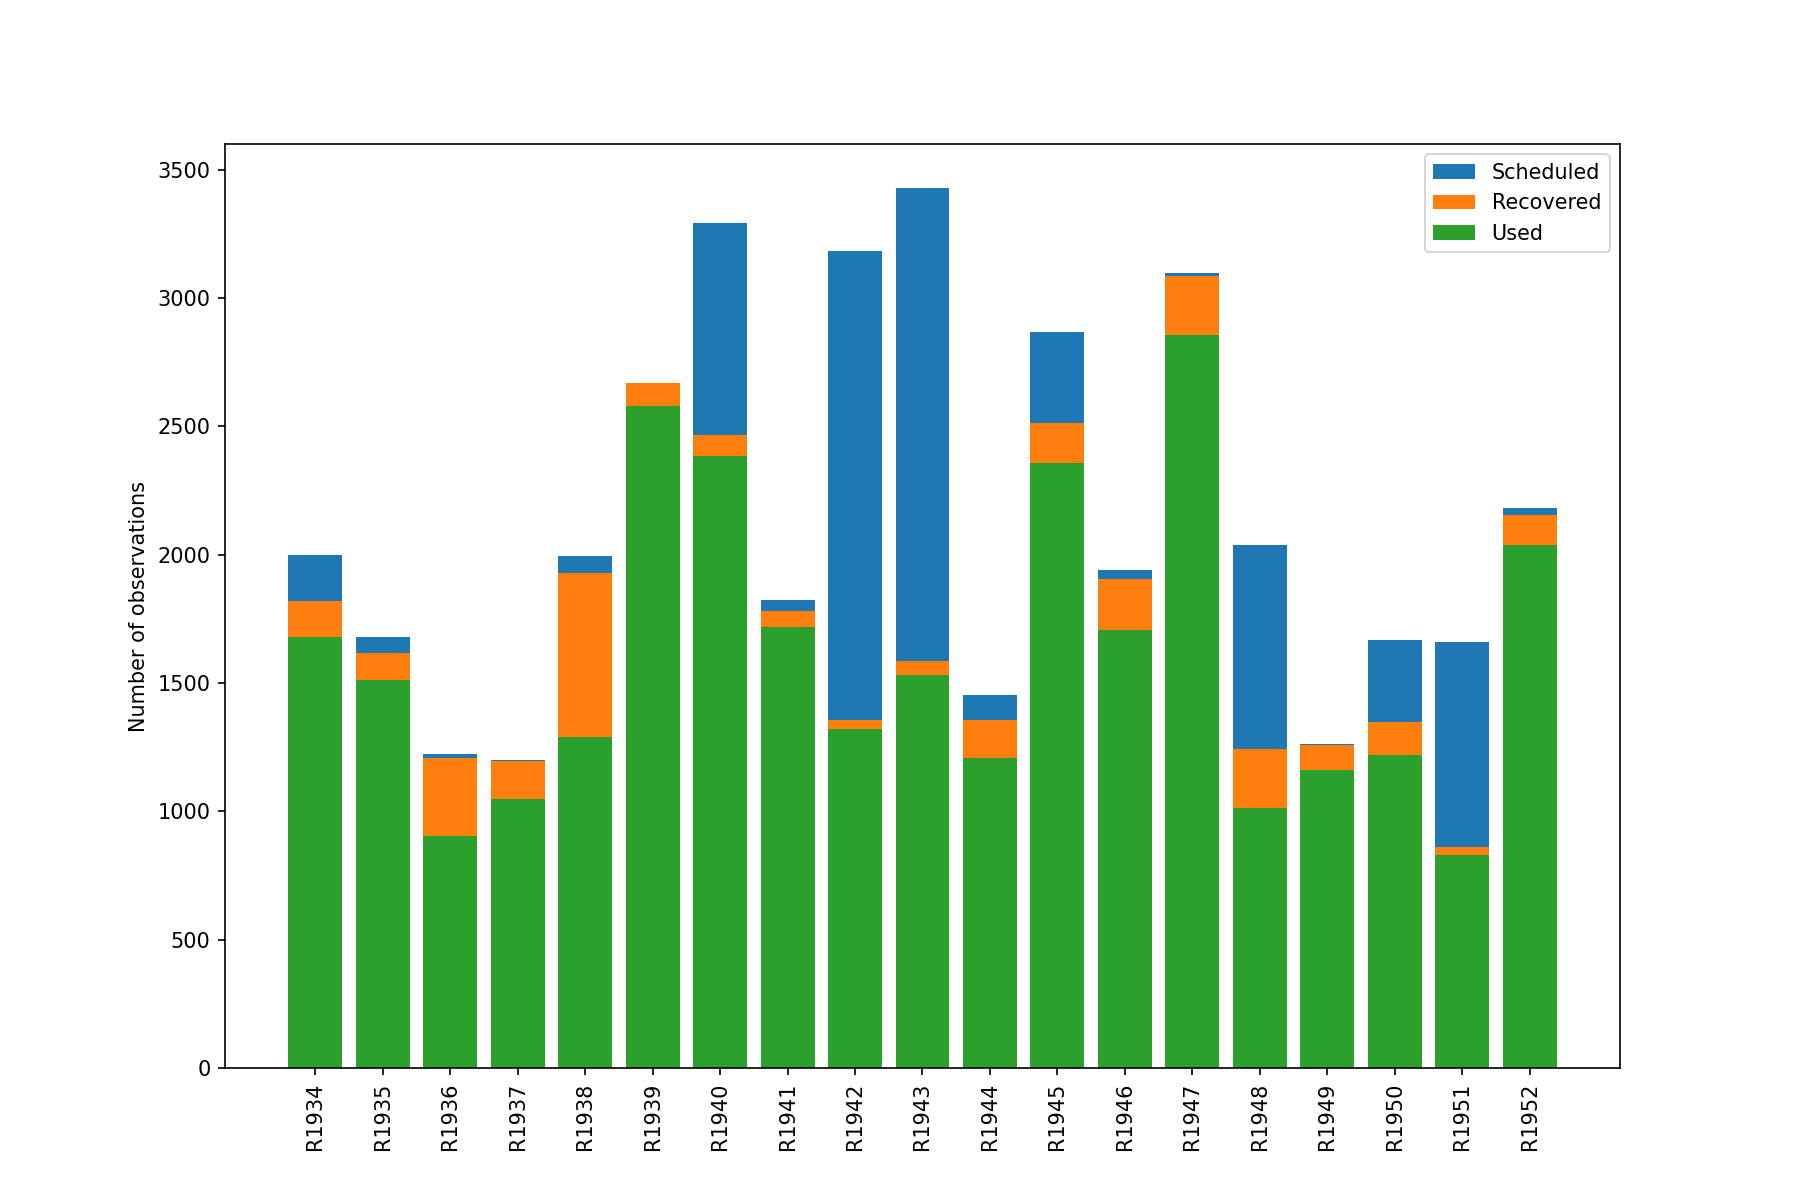
\includegraphics[width=0.5\linewidth]{figure/Num_obs_NYALES20_nyale13s9}} \\
    % Baseline lengths
	\subfloat[\textcolor{black}{Baseline length - NYALE13S/NYALES20 - Solution 0}.\label{fig:bl-0}]
      {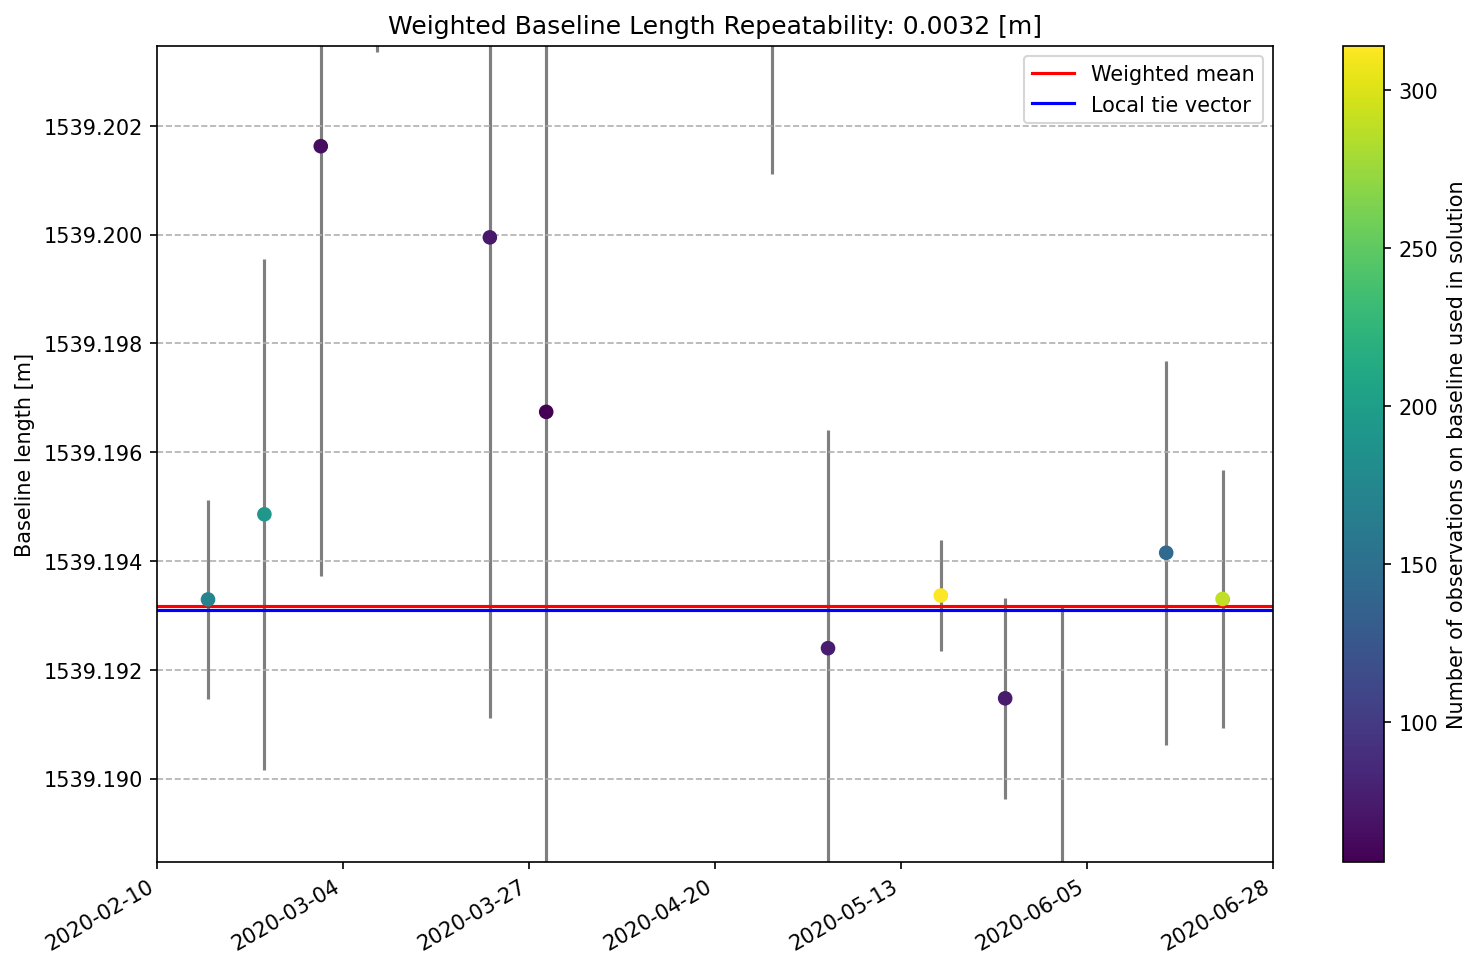
\includegraphics[width=0.5\linewidth]{figure/Baseline_NYALES20_NYALE13S_nyale13s0}}
	\subfloat[\textcolor{black}{Baseline length - NYALE13S/NYALES20 - Solution 9}.\label{fig:bl-9}]
      {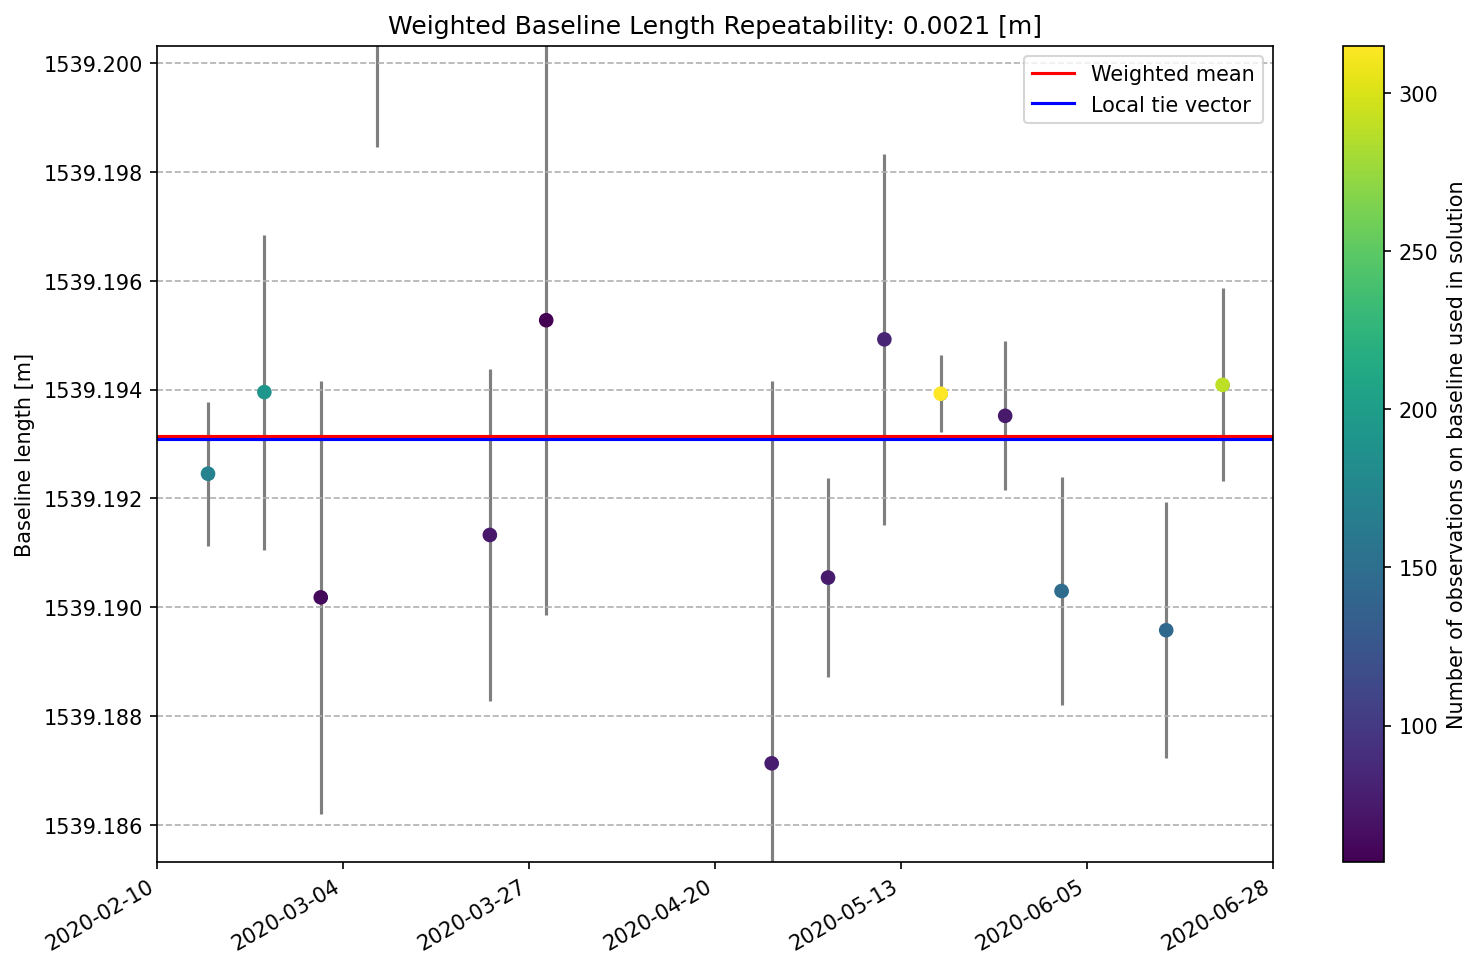
\includegraphics[width=0.5\linewidth]{figure/Baseline_NYALES20_NYALE13S_nyale13s9}} \\
    % Position NYALE13S
	\subfloat[\textcolor{black}{Estimated position - NYALE13S- Solution 0}.\label{fig:pos-Ns-0}]
      {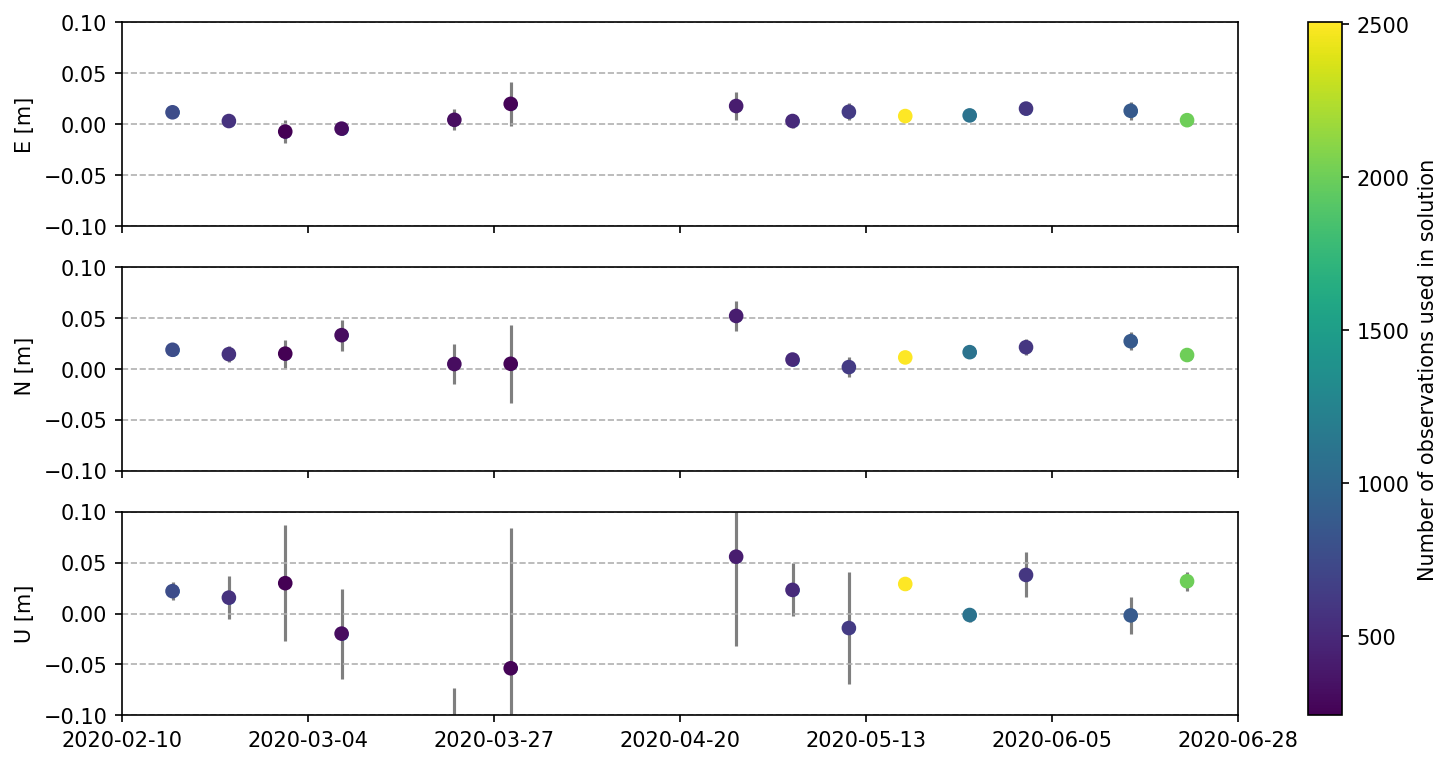
\includegraphics[width=0.5\linewidth]{figure/Position_NYALE13S_enu_nyale13s0}}
	\subfloat[\textcolor{black}{Estimated position - NYALE13S - Solution 9}.\label{fig:pos-Ns-9}]
      {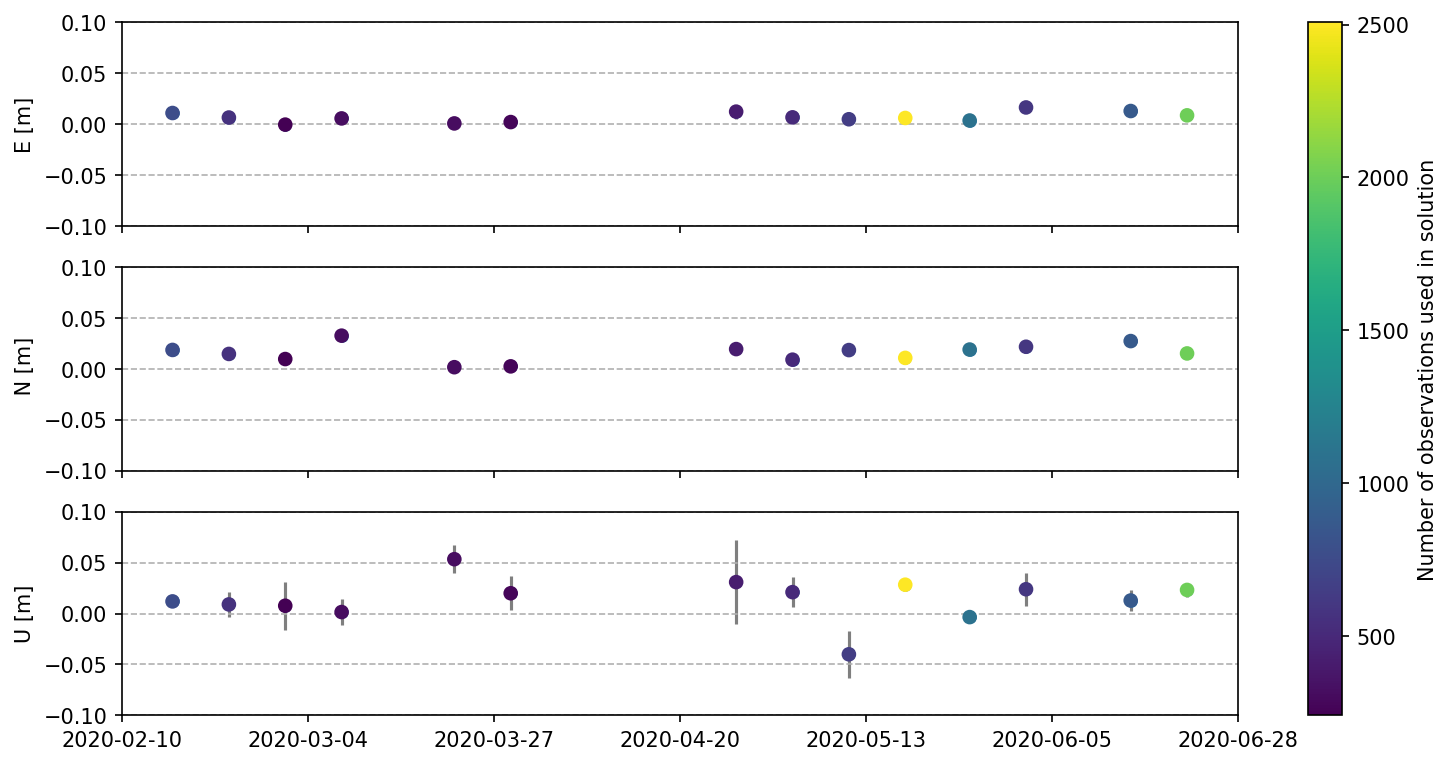
\includegraphics[width=0.5\linewidth]{figure/Position_NYALE13S_enu_nyale13s9}} \\
    % Position NYALES20
	\subfloat[\textcolor{black}{Estimated position - NYALES20 - Solution 0}.\label{fig:pos-Ny-0}]
      {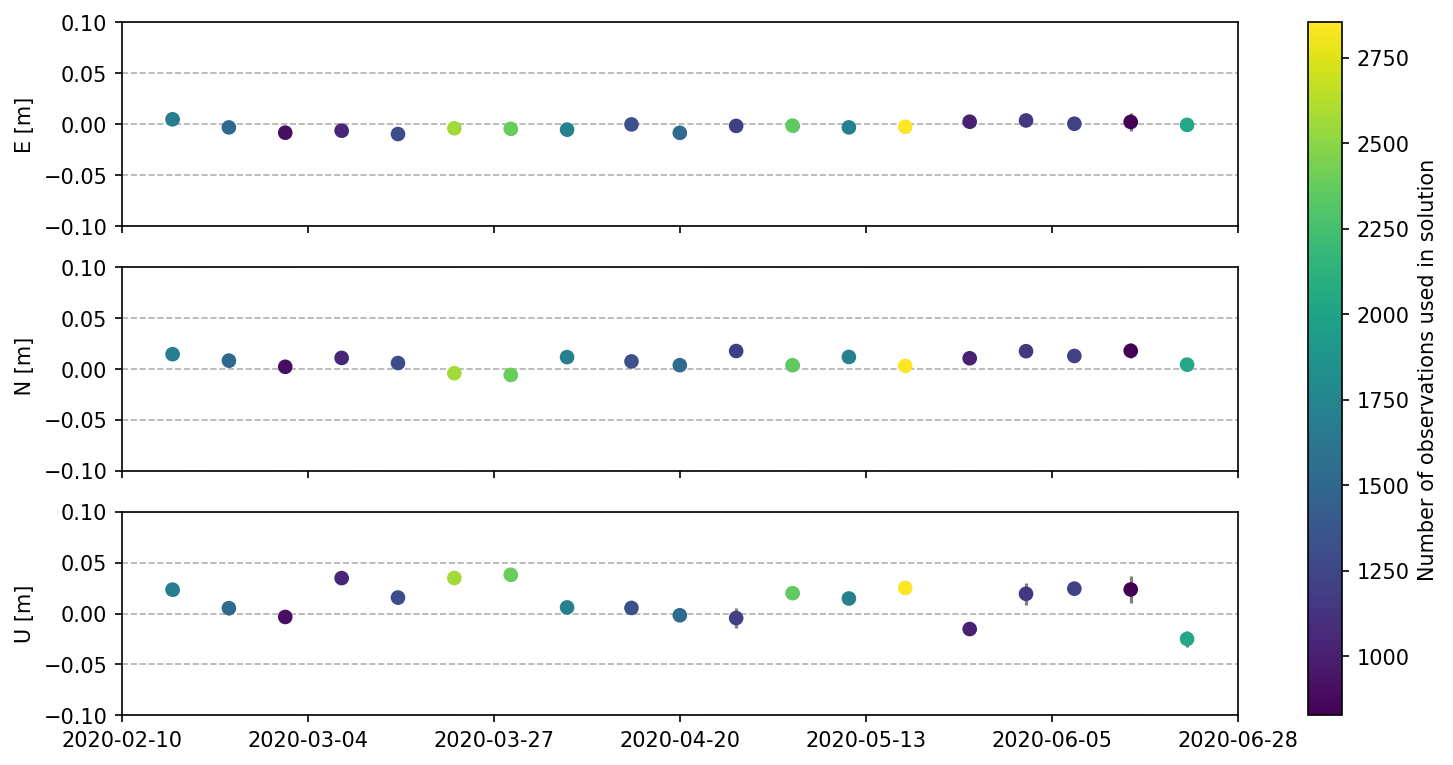
\includegraphics[width=0.5\linewidth]{figure/Position_NYALES20_enu_nyale13s0}}
	\subfloat[\textcolor{black}{Estimated position - NYALES20 - Solution 9}.\label{fig:pos-Ny-9}]
      {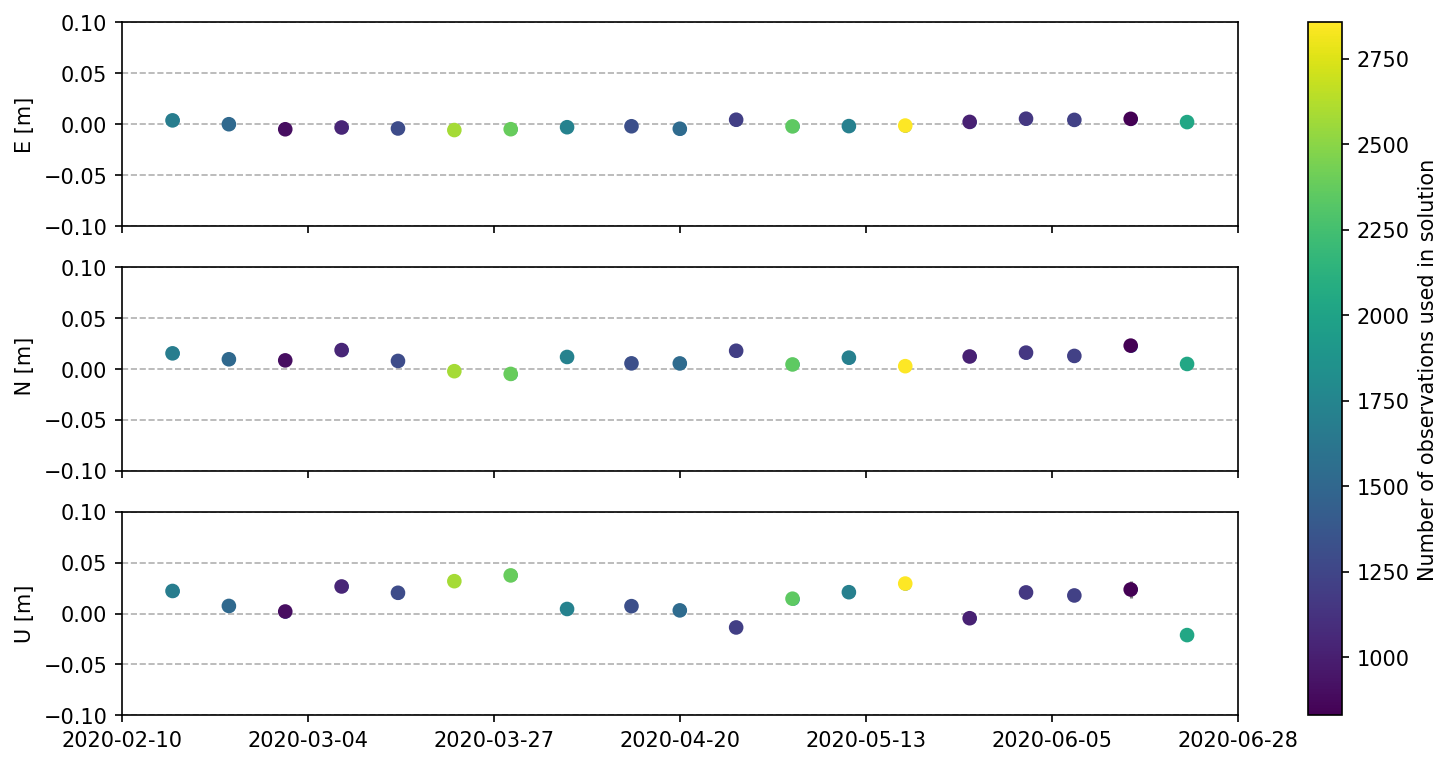
\includegraphics[width=0.5\linewidth]{figure/Position_NYALES20_enu_nyale13s9}} \\
    % RMS
	\subfloat[\textcolor{black}{Root mean square of postfit residuals [m] - Solution 0}.\label{fig:rms-0}]
      {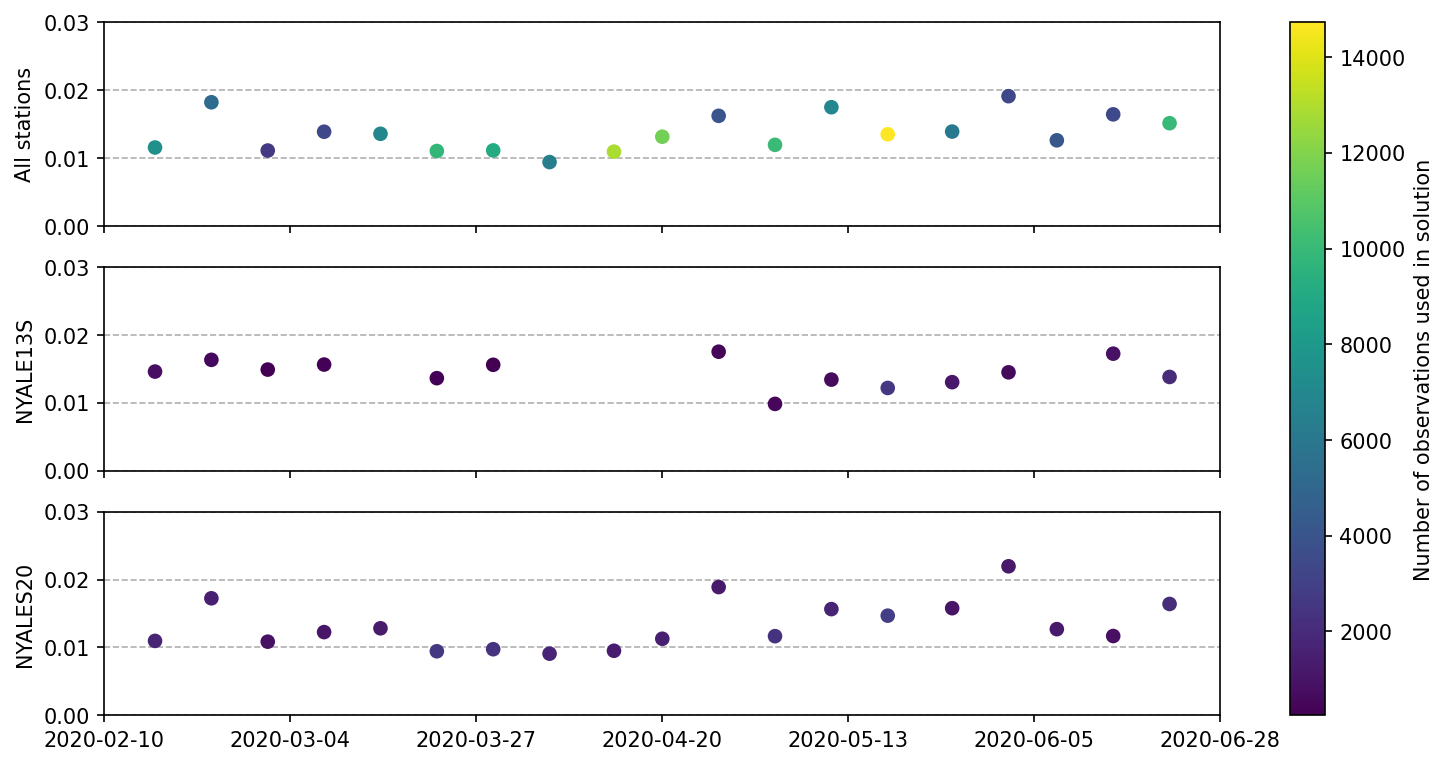
\includegraphics[width=0.5\linewidth]{figure/RMS_Postfit_Residuals_nyale13s0}}
	\subfloat[\textcolor{black}{Root mean square of postfit residuals [m] - Solution 9}.\label{fig:rms-9}]
      {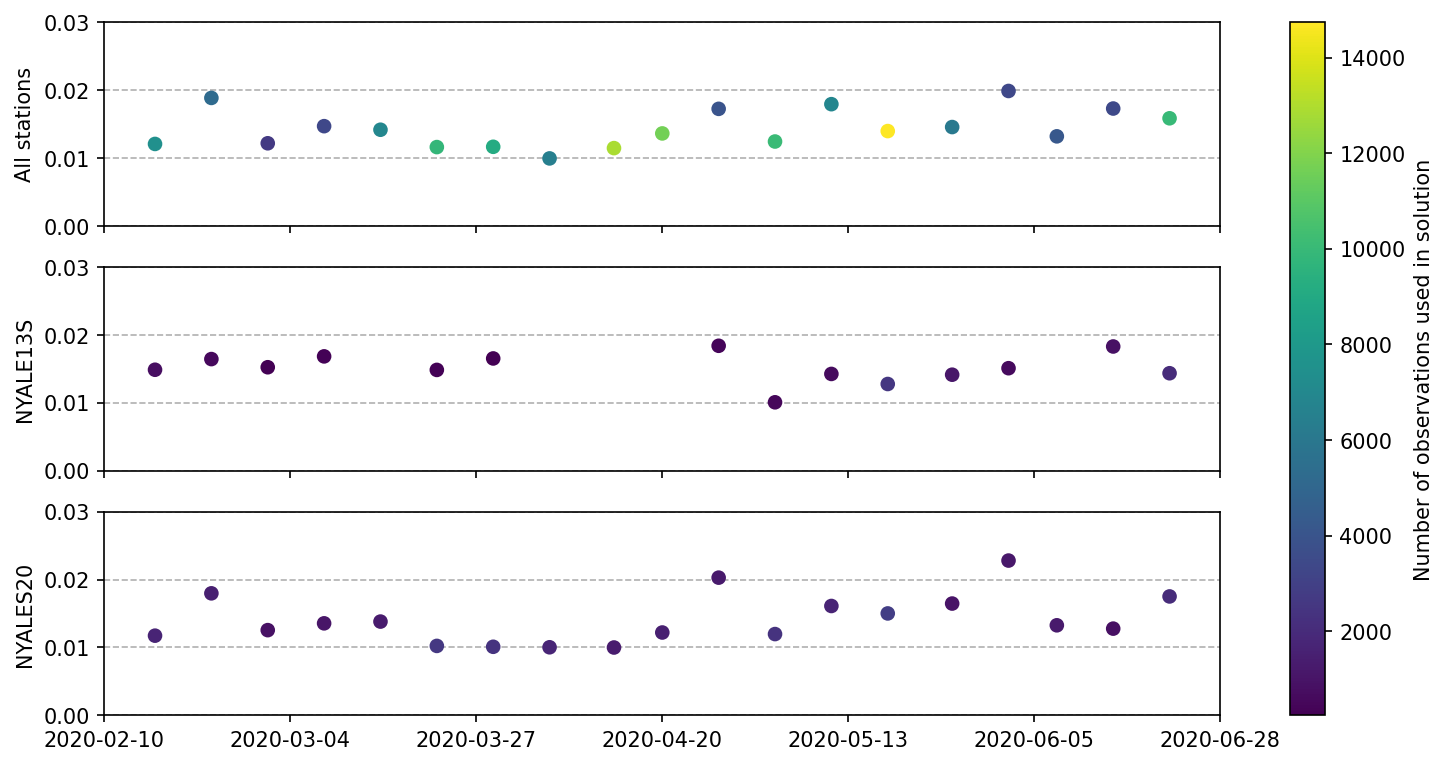
\includegraphics[width=0.5\linewidth]{figure/RMS_Postfit_Residuals_nyale13s9}} \\
    % Statistics
	\subfloat[\textcolor{black}{Statistics - Solution 0}.\label{fig:stat-0}]
      {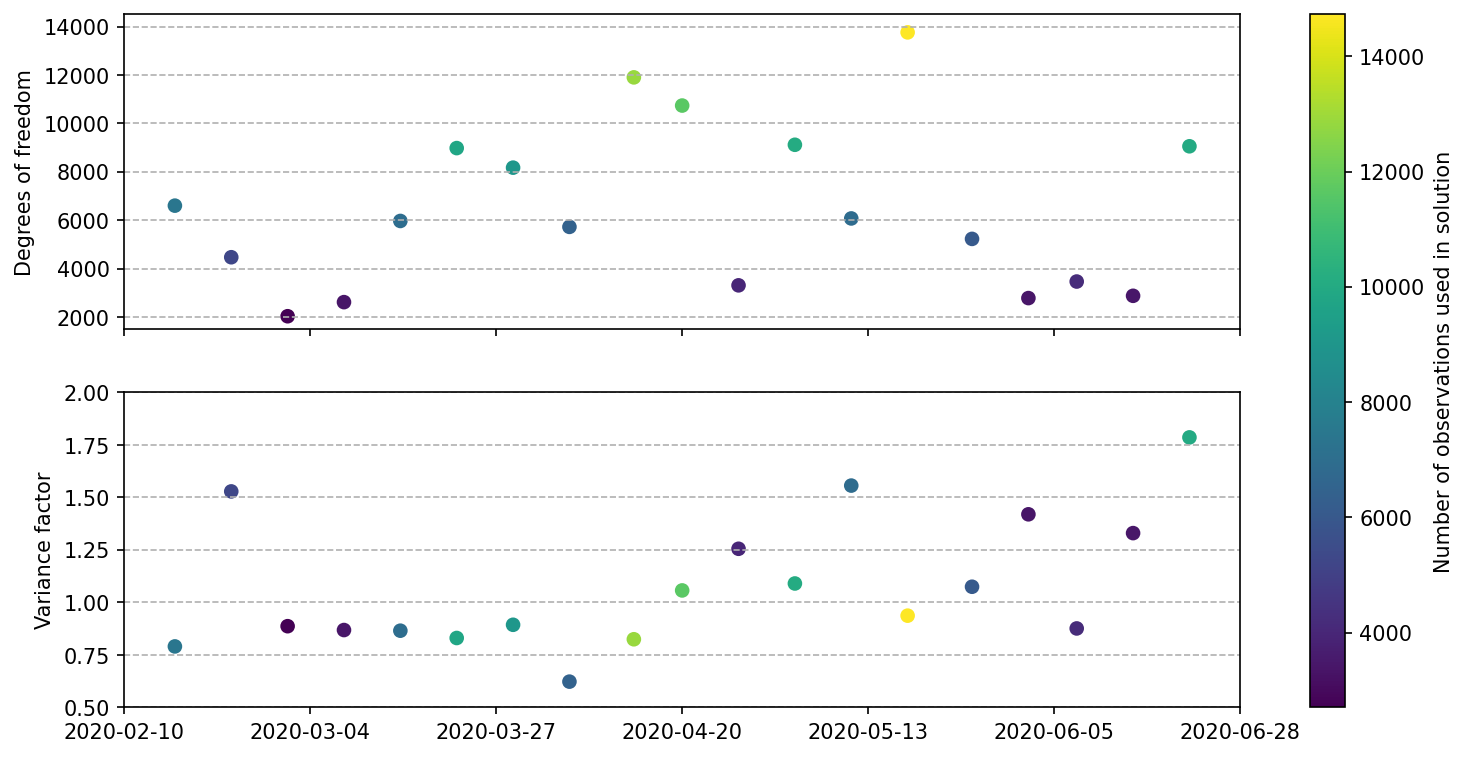
\includegraphics[width=0.5\linewidth]{figure/Statistics_nyale13s0}}
	\subfloat[\textcolor{black}{Statistics - Solution 9}.\label{fig:stat-9}]
      {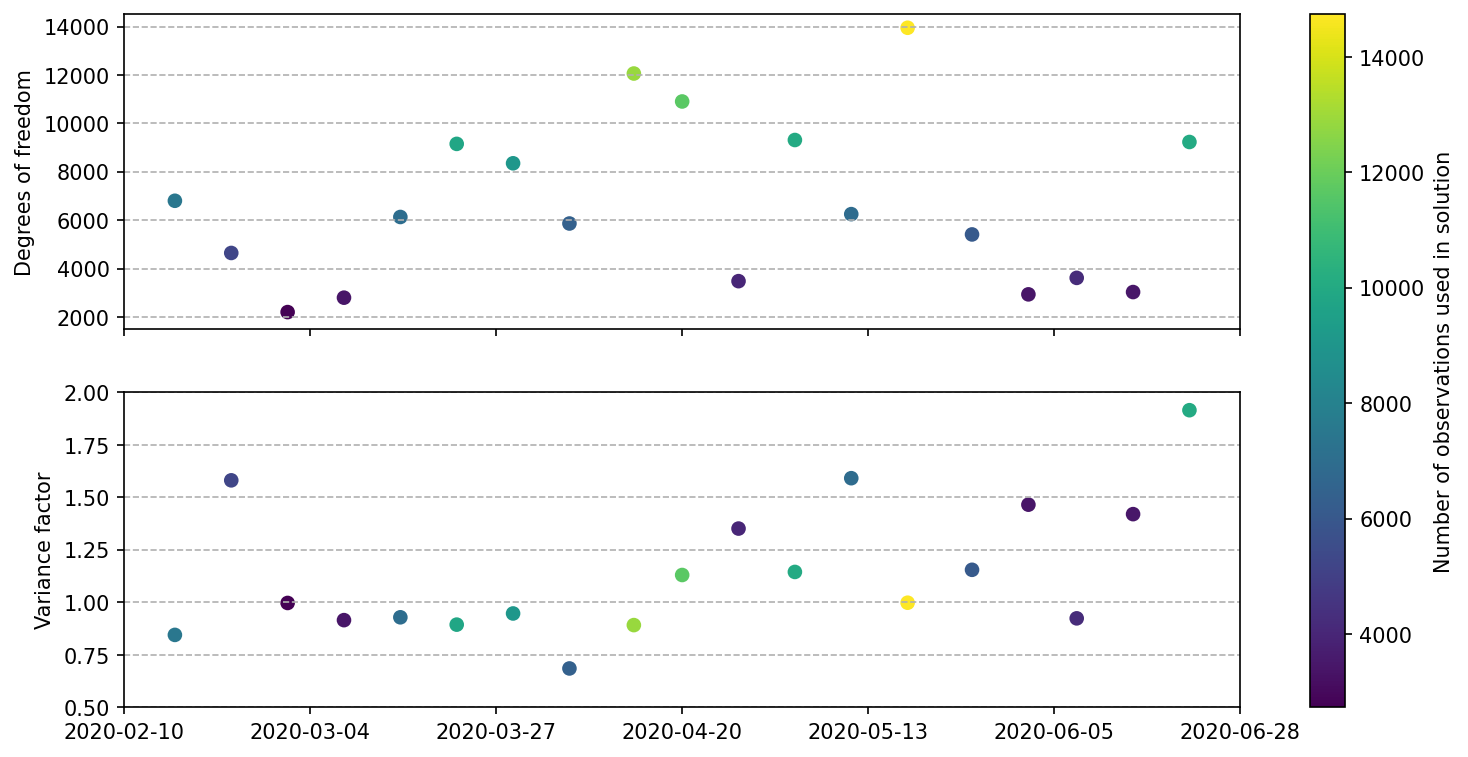
\includegraphics[width=0.5\linewidth]{figure/Statistics_nyale13s9}} \\
    %  
	\caption{Number of observations, estimated baseline length and positions for each session in addition to
	the postfit residuals and statistics for the sessions. The first column shows solution 0 and the second 
	solumn shows solution 9.}
	\label{fig:plots}
\end{figure}

\endinput
